\chapter{Experimentálny výskum} 

V tejto kapitole opisujem experimentálne porovnanie algoritmov na rôznych vstupných dátach. 

\section{Vstupné súbory}
Zdroje dát boli na realizáciu experimentálneho výskumu boli použité dáta z UMCI Machine Learning Repository \cite{bache2013}. 
Tieto dáta sú využívané na experimentálne porovnania metód a algoritmov získania znalostí.
Pre realizáciu experimentov boli použité súbory, ktorých výstupný atribút nadobúda hodnoty z konečnej množiny celočíselných hodnôt. 

V experimentov som použila nasledovné súbory, ktorých súbor dát obsahuje: 
\begin{itemize}
	\item \textbf{Iris}  - výsledky merania parametrov kvetov kosatcov. Výstupný atribút je typ jedného z troch druhov kvetov.  
	\item \textbf{Heart} - výsledky merania  rôznych ukazovateľov pacientov, trpiacich na srdcovo-cievne ochorenie. Výsledný atribút opisuje stupeň vážnosti ochorenia. 
	\item \textbf{Seeds} - dáta získané ako výsledok merania geometrických vlastností zŕn troch rozličných odrôd pšenice v Inštitúte geofyziky Poľskej akadémie vied. 
	
	\item \textbf{Wine} - dáta chemických ukazovateľov rôznych druhov juhotalianských vín. Vstupné atribúty obsahujú ingrediencie vo víne. Výstupný atribút určuje jeden z troch druhov vína. 
	
	\item \textbf{Yeast} - slúži na predikciu umiestnenia proteínov v bunkách kvasiniek. 

\end{itemize}


Základné charakteristiky vybraných súborov sú: 

\begin{itemize}
 \item počet pozorovaní, 
 \item počet vstupných atribútov, nadobúdajúcich lingvistické alebo číselné hodnoty, 
 \item počet variantov výstupného atribútu, 
 \item hodnota počiatočnej chyby výberu. 
\end{itemize}


V tabuľke č. \ref{table:suborydat} sú hodnoty charakteristík vybraných súborov dát.


\begin{table}[h!]
	\centering
\begin{tabular}{|p{1,4cm}|p{2cm}|p{2cm}|p{2,35cm}|p{2cm}|p{2,2cm}|p{2cm}|}
	\hline 
	
	Súbor dát & Počet  \mbox{pozorovaní} & Počet \mbox{výstupných} atribútov&
   Počet \mbox{lingvistických} atribútov&
    Počet \mbox{číselných} atribútov& 	
	P. variantov výstupného atribútov  & \mbox{Počiatočná} chyba výberu \\ 
	\hline 
	
	Heart & 270 & 13 &8& 5 & 2 & 0,4444 \\ 
	\hline 
	Iris & 150 & 4 &0 &4& 3 & 0,6667 \\ 
	\hline 
	Seeds & 210 & 7&0 & 7 & 3 & 0,3490 \\ 
	\hline 
	Wine & 178 & 13&0&13& 3 & 0,6011 \\ 
	\hline 
	Yeast & 1484 & 8 &2& 6 & 10 & 0,6880 \\ 
	\hline 	
\end{tabular} 
	\caption{Hodnoty charakteristík vybraných súborov dát.}
\label{table:suborydat}
\end{table}


\section{Súbor údajov Iris}

\subsection{Opis vstupných dát}
Je to najznámejšia databáza, ktorá sa nachádza v literatúre rozpoznávania vzorov. Súbor údajov obsahuje 3 triedy po 50 prípadoch, kde každá trieda sa vzťahuje na typ rastliny dúhovky. Jedna trieda je lineárne oddeliteľná od ostatných 2; Tieto nie sú lineárne oddeliteľné od seba. 
%todo citovat Https://archive.ics.uci.edu/ml/datasets/Iris

Prvé atribút je dĺžka sepálu v cm, druhý atribút je šírka sepálu v cm, tretí atribút dĺžka okvetných lístkov v cm, štvrtý atribút je šírka okvetných lístkov v cm. Výstupný atribút má triedy - Iris Setosa, Iris Versicolour, Iris Virginica. 

\begin{table}[h!]
\centering

\label{suhrne-statistiky-iris}
\begin{tabular}{|l|l|l|l|l|l|}
\hline
\textbf{Atribút} & \textbf{Min} & \textbf{Max} & \textbf{Mean} & \textbf{SD} & \textbf{Korelácia} \\ \hline
Dĺžka sepálu & 4,3 & 7,9 & 5,84 & 0,83 & 0,7826 \\ \hline
Šírka sepálu & 2,0 & 4,4 & 3,05 & 0,43 & -0,4194 \\ \hline
Dĺžka okvetného lístka & 1,0 & 6.9 & 3.76 & 1.76 & 0.9490 \\ \hline
Šírka okvetného lístka & 0.1 & 2.5 & 1.20 & 0.76 & 0.9565 \\ \hline
\end{tabular}
\caption{Súhrnné štatistiky pre databázu Iris}
\end{table}
\subsection{Výsledky fuzzifikácie}

Výsledky fuzzifikácie sú v tabuľke č.\ref{vysledky-tabulka-iris}. V tabuľke som vybrala som hodnotu entropiu pre atribút prvý a umiestnenie centier pre atribút štvrtý.  
\begin{table}[]
\centering
\label{vysledky-tabulka-iris}
\begin{tabular}{|l|c|c|l|}
\hline
\textbf{} & \textbf{Počet intervalov} & \textbf{\begin{tabular}[c]{@{}c@{}}Hodnota entropie \\ pre atribút 1\end{tabular}} & \multicolumn{1}{c|}{\textbf{\begin{tabular}[c]{@{}c@{}}Umiestnenie \\ centier pre atribút 4\end{tabular}}} \\ \hline
\textbf{Algoritmus 1} & 2,2,3,3,3 & 4,4680315 & 0,0600  0,5154   0,8225 \\ \hline
\textbf{Algoritmus 2} & 2,2,5,3,3 & 2,2678531 & 0,0600 0,5154  0,8225 \\ \hline
\textbf{Algoritmus 3} & 3,3,4,4,3 & 6,8543783 & 0,0600  0,4722  0,6595  0,8822 \\ \hline
\textbf{Algoritmus 4} & 5,2,3,4,3 & 1,6914607 & 0,0000  0,0417 0,3750  0,4583 \\ \hline
\end{tabular}
\caption{Výsledky fuzzifikácie Iris databázy.}

\end{table}

\subsection{Experiment - Vývoj hodnoty entropie }
Experiment spočíva v sledovaní vývoja hodnoty entropie prvého atribútu v  intervale $<2,22>$. Hodnota entropie pri Algoritme 1 stúpa, zatiaľ čo algoritmy čo používajú váženú entropiu, sa hodnoto udržujú na rovnakej úrovni.  Počet tried na intervale tri je priemerne pre triedy 60, 60, 30. 
\begin{figure}[ht!]
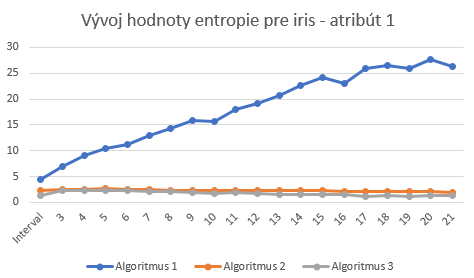
\includegraphics[width=0.75\textwidth]{obrazky/iris-vyvoj-entropie-atribut1.PNG}
\centering
\caption{Vývoj hodnoty entropie pre iris - atribút 1. } 
\label{fig:structure}
\end{figure}

\section{Súbor údajov vína}

\subsection{Opis vstupných dát}
Tieto údaje sú výsledkom chemickej analýzy vín pestovaných v rovnakom regióne v Taliansku, ale odvodených od troch rôznych kultivarov. Analýza určila množstvo 13 zložiek, ktoré sa nachádzajú v každom z troch druhov vín. 
%https://archive.ics.uci.edu/ml/datasets/Wine

 Počet inštancií je 178, z toho v triedach je 59, 71, 48 položiek.  Prvý atribút je identifikátor triedy. Počet atribútov má 4 číselných, 1 prediktívný atribút a triedu. 
Názvy atribútov: Alkohol , Kyselina jablčná, Popol 
, Alkalinity popola 
, Horčík 
, Celkové fenoly 
, Flavanoidy
, Neflavanoidné fenoly
, Proantokyaníny 
, Intenzita farieb
, Odtieň 
, OD280 / OD315 zriedených vín 
, Prolín. 



\subsection{Výsledky fuzzifikácie a experimenty}
Výsledky fuzzifikácie sú v tabuľke č.\ref{vysledky-tabulka-wine}. Počet tried pre atribút prvý je 61, 56, 61. 
Experiment spočíva v sledovaní vývoja hodnoty entropie prvého atribútu. 

\begin{table}[]
\centering

\label{vysledky-tabulka-wine}
\begin{tabular}{|l|c|l|l|}
\hline
\textbf{} & \textbf{\begin{tabular}[c]{@{}c@{}}Hodnota entropie \\ pre atribút 1\end{tabular}} & \textbf{\begin{tabular}[c]{@{}l@{}}Hodnota entropie \\ pre atribút 1  ($I+1$) \end{tabular}} & \multicolumn{1}{c|}{\textbf{\begin{tabular}[c]{@{}c@{}}Umiestnenie centier\\ pre atribút 1\end{tabular}}} \\ \hline
\textbf{Algoritmus 1} & 4,8846493 & 7,6232103 & 0,3289  0,6919 \\ \hline
\textbf{Algoritmus 2} & 2,7733194 & 2,8339819 & 0,3289 0,6919 \\ \hline
\textbf{Algoritmus 3} & 4,8846493 & 7,6232103 & 0,2779 0,5232 0,7550 \\ \hline
\textbf{Algoritmus 4} & 1,1502002 & 2,1532059 & 0,1395 0,1553 \\ \hline
\end{tabular}
\caption{Výsledky fuzzifikácie Wine databázy.}
\end{table}

\begin{figure}[ht!]
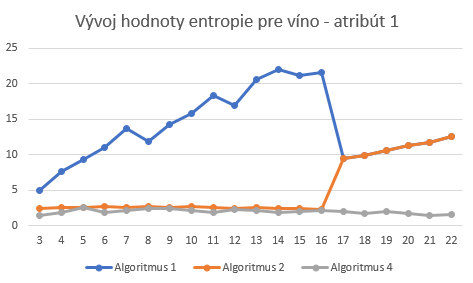
\includegraphics[width=0.75\textwidth]{obrazky/wine-vyvoj-entropie-atribut1.PNG}
\centering
\caption{Vývoj hodnoty entropie pre víno - atribút 1} 
\label{fig:structure}
\end{figure}

\section{Súbor údajov kvasníc (Yeast)}
%https://archive.ics.uci.edu/ml/datasets/Yeast
Údaje sú na predpovedanie bunkovej lokalizácie proteínov. 
Počet inštancií je  1484 pre súbor údajov o kvasinkách.
 Počet atribútov pre súbor kvasiniek je 9 (8 prediktívnych, 1 názov): 
\begin{enumerate}
\item Názov série: Prístupové číslo pre databázu SWISS-PROT
\item mcg: McGeochova metóda na rozpoznávanie signálových sekvencií.
\item gvh: von Heijneov metóda pre rozpoznávanie signálnej sekvencie.
\item alm: Skóre prognózového programu ALOM membránovej oblasti.
\item mit: Skóre analýzy obsahu aminokyselín.
\item erl: Prítomnosť substringu "HDEL". Binárny atribút.
\item pox: Peroxizomálny cieľový signál na C-konci.
\item vac: Skóre rozlišovacej analýzy obsahu aminokyselín v
Vakuolárne a extracelulárne proteíny.
\item nuc: Skóre analýzy jadrových lokalizačných signálov.

\end{enumerate}
 Distribúcia tried je nasledovná : 
\begin{itemize}
\item CYT (cytosolický alebo cytoskeletálny) - 463
\item NUC (nukleárne)  - 429
\item MIT (mitochondriálna)  - 244
\item ME3 (membránový proteín, žiadny N-koncový signál) -  163
\item ME2 (membránový proteín, neštiepený signál)  - 51
\item ME1 (membránový proteín, štiepený signál)  - 44
\item EXC (extracelulárne)  - 37
\item VAC (vakuolárne)  - 30
\item POX (peroxisomálny) - 20
\item ERL (endoplazmatický retikulový lumen) -  5
\end{itemize}
Výsledky fuzzifikácie sú v tabuľke č. \ref{my-label44}
\begin{table}[hp!]
\centering
\begin{tabular}{|l|c|l|l|}
\hline
\textbf{} & \textbf{\begin{tabular}[c]{@{}c@{}}Hodnota entropie \\ pre atribút 1\end{tabular}} & \textbf{\begin{tabular}[c]{@{}l@{}}Hodnota entropie \\ pre atribút 1 - I+1\end{tabular}} & \multicolumn{1}{c|}{\textbf{\begin{tabular}[c]{@{}c@{}}Umiestnenie centier\\ pre atribút 1\end{tabular}}} \\ \hline
\textbf{Algoritmus 1} & 4,8846493482439 & 7,6232103794469 & 0,3289  0,6919 \\ \hline
\textbf{Algoritmus 2} & 2,77331942036114 & 2,83398191261714 & 0,3289 0,6919 \\ \hline
\textbf{Algoritmus 3} & 4,8846493482439 & 7,6232103794469 & 0,2779 0,5232 0,7550 \\ \hline
\textbf{Algoritmus 4} & 1,15020020568059 & 2,15320594479199 & 0,1395 0,1553 \\ \hline
\end{tabular}
\caption{Výsledky fuzzifikácie pre súbor dát kvasníc}
\label{my-label44}
\end{table}

\section{Súbor údajov Statlog (srdce)}
%Https://archive.ics.uci.edu/ml/datasets/Statlog+%28Heart%29
Táto sada dát je databáza srdcových ochorení. Počet inštancií je 270 a atribútov je 13.  Predpokladaná premenná je absencia (1) alebo prítomnosť (2) ochorenia srdca.
Typy atribútov:
\begin{itemize}
\item Numerické: 1,4,5,8,10,12. 
\item Usporiadané: 11. 
\item Binárne: 2,6,9. 
\item Nominálna hodnota: 7,3,13.
\end{itemize}
V tabuľke č. \ref{my-label45} sú výsledky fuzzifikácie dát. 

\begin{table}[hp!]
\centering
\begin{tabular}{|l|c|l|l|}
\hline
\textbf{} & \textbf{\begin{tabular}[c]{@{}c@{}}Hodnota entropie \\ pre atribút 1\end{tabular}} & \textbf{\begin{tabular}[c]{@{}l@{}}Hodnota entropie \\ pre atribút 1 - I+1\end{tabular}} & \multicolumn{1}{c|}{\textbf{\begin{tabular}[c]{@{}c@{}}Umiestnenie centier\\ pre atribút 1\end{tabular}}} \\ \hline
\textbf{Algoritmus 1} & 4,8846493482439 & 7,6232103794469 & 0,3289  0,6919 \\ \hline
\textbf{Algoritmus 2} & 2,77331942036114 & 2,83398191261714 & 0,3289 0,6919 \\ \hline
\textbf{Algoritmus 3} & 4,8846493482439 & 7,6232103794469 & 0,2779 0,5232 0,7550 \\ \hline
\textbf{Algoritmus 4} & 1,15020020568059 & 2,15320594479199 & 0,1395 0,1553 \\ \hline
\end{tabular}
\caption{Výsledky fuzzifikácie pre súbor dát srdce}
\label{my-label45}
\end{table}

\section{Súbor dát semien}
%https://archive.ics.uci.edu/ml/datasets/seeds
 Súbor dát je z merania geometrických vlastností jadier, ktoré patria do troch rôznych odrôd pšenice. Mäkká röntgenová technika a balík GRAINS boli použité na zostavenie všetkých siedmich atribútov s reálnou hodnotou.
 
 Informácie o atribútoch: Na zostrojenie údajov sa meralo sedem geometrických parametrov pšeničných jadier: 
oblasť A, 
obvod P, 
kompaktnosť C = $4 * pi * A / P ^ 2$, 
 dĺžka jadra, 
 šírka jadra, 
 koeficient asymetrie, 
dĺžka drážky jadra. 

V nasledujúcej tabuľke \ref{my-label33} sú výsledky pre súbor dát semien. 

\begin{table}[hp!]
\centering
\begin{tabular}{|l|c|l|l|}
\hline
\textbf{} & \textbf{\begin{tabular}[c]{@{}c@{}}Hodnota entropie \\ pre atribút 1\end{tabular}} & \textbf{\begin{tabular}[c]{@{}l@{}}Hodnota entropie \\ pre atribút 1\end{tabular}} & \multicolumn{1}{c|}{\textbf{\begin{tabular}[c]{@{}c@{}}Umiestnenie centier\\ pre atribút 1\end{tabular}}} \\ \hline
\textbf{Algoritmus 1} & 4,8846493482439 & 7,6232103794469 & 0,3289  0,6919 \\ \hline
\textbf{Algoritmus 2} & 2,77331942036114 & 2,83398191261714 & 0,3289 0,6919 \\ \hline
\textbf{Algoritmus 3} & 4,8846493482439 & 7,6232103794469 & 0,2779 0,5232 0,7550 \\ \hline
\textbf{Algoritmus 4} & 1,15020020568059 & 2,15320594479199 & 0,1395 0,1553 \\ \hline
\end{tabular}
\caption{Výsledky fuzzifikácie pre súbor dát - Semená}
\label{my-label33}
\end{table}

\section{Zhrnutie výsledkov }
Algoritmus 4 efektívne zoradí centra. Pri Algoritme 1 hodnota entropie stúpa smerom nahor. Algoritmus 2 pomocou váženej entropie je dobrý na určenie počtu intervalov, ak triedy majú nerovnomerne rozdelené prvky. Algoritmus 3 dáva vyšší počet intervalov kvôli tomu, že prahová hodnota bola nastavená nízko. 



%\section{Parametre, určujúce kvalitu fuzzifikácie}
%
%\section{Priebeh experimetnov - použité dátové množiny}
%
%\section{Výsledky a vyhodnotenie experimentov pre vybraté dátové množiny}
%
%\section{Zhrnutie výsledkov }
%
%\section{Záver}